\documentclass[a4paper, 10pt]{article}
\usepackage[utf8]{inputenc} % Change according your file encoding
\usepackage{graphicx}
\usepackage{url}
\usepackage{amsmath}
\usepackage{mathtools}
\usepackage{mathrsfs}
\usepackage{amsfonts}
\usepackage{bbm}
\usepackage{amsthm}
\usepackage{amssymb}
\usepackage{fancyhdr}
\usepackage{setspace}
\usepackage{tabularx}
\usepackage{tcolorbox}
\usepackage{tikz}
\usepackage[a4paper, left=2cm, right=2cm, top=2.5cm, bottom=2cm]{geometry}
\usepackage[ruled]{algorithm2e}

% Links, link colors, and clickable ToC
\usepackage{hyperref}
\hypersetup{
    colorlinks,
    citecolor=black,
    filecolor=black,
    linkcolor=black,
    urlcolor=black
}

\pagestyle{fancy}
\fancyhf{}
\rhead{Group 2 - Problem \thesection}
\lhead{M. Altarriba, E. Gonzalvo, A. Mir, C. Segarra}
\cfoot{\thepage}

% New commands
\newcommand{\Z}{\mathbb{Z}}
\newcommand{\F}{\mathbb{F}}
\newcommand\tab[1][1cm]{\hspace*{#1}}
\renewcommand{\P}{\mathcal{P}}

\newtheorem{obs}{Observation}
\newtheorem{theorem}{Theorem}
\newtheorem*{theoremstar}{Theorem}

\theoremstyle{definition} % amsthm only
\newtheorem{definition}{Definition}

\begin{document}
\onehalfspacing
\pagestyle{empty}

\begin{center}
    \vspace{2cm}
    \includegraphics[width=8cm]{img/logo_fme.png}
    \vspace{2cm}

    \Large
    Master in Advanced Mathematics and Mathematical Engineering
    \vspace{0.5cm}

    \LARGE
    Codes \& Cryptography: Problem Assignment - Group 2

    \vspace{0.5cm}
    \large
    Marta Altarriba, Eduard Gonzalvo, Arnau Mir, Carlos Segarra

    \vspace{0.5cm}
    \normalsize
    \today

    \vspace{1cm}

\end{center}

\tableofcontents


\newpage
\pagestyle{fancy}
\section{Problem 1:}\label{sec:problem1}

Suppose $F$ is a secure PRP with blocklength $\lambda$. Give the decryption algorithm for the following scheme and prove that it does not have CPA security:

\newpage
\section{Problem 2: Simple PRF from DDH}\label{sec:problem2}

Let $\mathbb{G}$ be a cyclic group of prime order $q$ generated by $g \in \mathbb{G}$.
Let $H : \mathcal{M} \rightarrow \mathbb{G}$ be a hash function, which we shall model as a random oracle.
Let $F$ be the PRF defined over $(\mathbb{Z}_{q},\mathcal{M},\mathbb{G})$ as follows:
\begin{equation*}
    F(k,m) \coloneqq H(m)^{k} \hspace{8pt} \text{for } k \in \mathbb{Z}_{q}, m \in \mathcal{M}.
\end{equation*}
Show that $F$ is a secure PRF in the random oracle model for $H$ under the DDH assumption for $\mathbb{G}$.
In particular, you should show that for every adversary $\mathcal{A}$ attacking $F$ as a PRF, there exists a DDH adversary $\mathcal{B}$, which is an elementary wrapper around $\mathcal{A}$, such that $PRFadv[\mathcal{A}, F] \leq DDHadv[\mathcal{B}, \mathbb{G}] + \frac{1}{q}$.

\begin{center}
    \rule{5cm}{0.4pt}
\end{center}

\textbf{\textit{Proof:}}
To solve this exercise we will see that if we can break the PRF game then two distributions are not computationally indistinguishable, and following the result from Exercise 10.10, the DDH assumption does not hold.
In particular, we play the attacker role in the PRF game as defined in \hyperref[ag:4-2]{Attack Game 4.2} and will leverage an adversary for the distinguishing game as defined in \hyperref[ag:3-3]{Attack Game 3.3}.

Let us define define, using the notation from Exercise 10.10, the following variables for the random distributions:
\begin{equation*}
    \begin{split}
        g^{a_i} = H(m) = g^x \text{ for some $x$, } \hspace{3pt} \beta_i = k \in \mathbb{Z}_q, \text{ and } \hspace{3pt} \gamma_i \text{ random}.
    \end{split}
\end{equation*}
The complete scheme is depicted in Figure~\ref{p2:ag}.

\begin{figure}[h!]
    \centering
    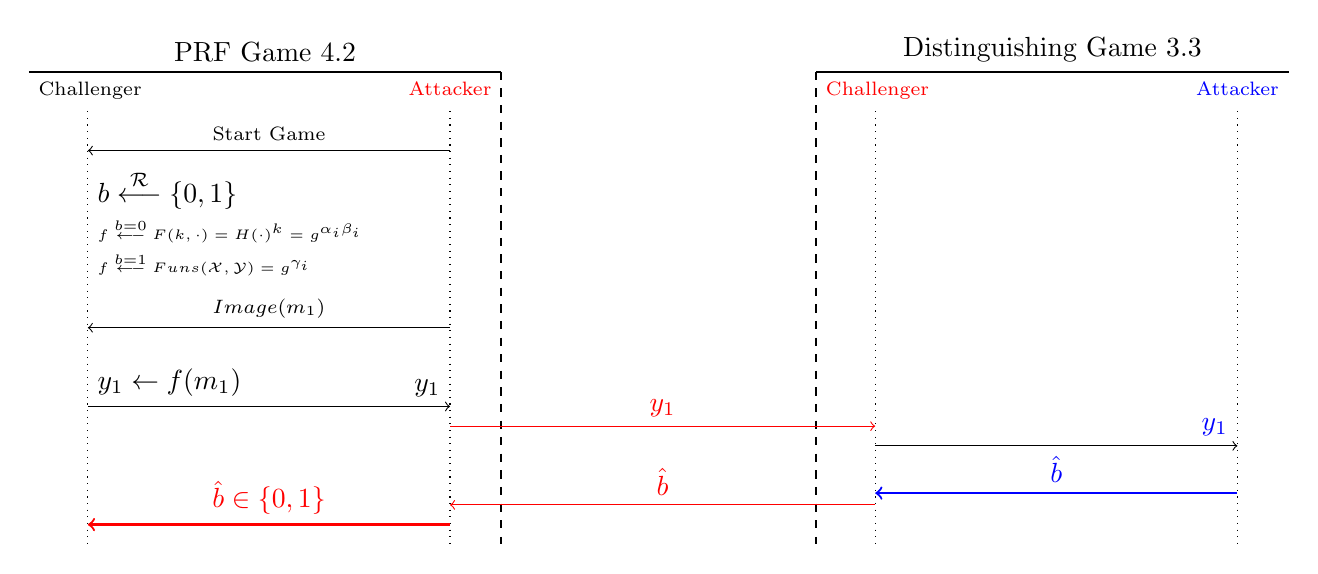
\begin{tikzpicture}
        % Define Variables
        \def\lR{0.75}
        \def\rR{5.35}
        \def\lDR{10.75}
        \def\rDR{15.35}
        \def\bottom{-6}

        % Overall Scheme
        \draw[thick] (0,0) -- (6,0) node[midway, anchor=south] {PRF Game $4.2$};
        \node[anchor = north west] at (0,0) (c-r) {\scriptsize Challenger};
        \draw[dotted] (\lR, -0.5) -- (\lR,\bottom);
        \node[anchor = north east, text=red] at (6,0) {\scriptsize Attacker};
        \draw[dotted] (\rR, -0.5) -- (\rR, \bottom);
        \draw[thick, dashed] (6,0) -- (6, \bottom);
        \draw[thick] (10,0) -- (16,0) node[midway, anchor=south] {Distinguishing Game $3.3$};
        \node[anchor = north west, text=red] at (10,0) {\scriptsize Challenger};
        \node[anchor = north east, text=blue] at (16,0) {\scriptsize Attacker};
        \draw[thick, dashed] (10,0) -- (10, \bottom);
        \draw[dotted] (\lDR, -0.5) -- (\lDR, \bottom);
        \draw[dotted] (\rDR, -0.5) -- (\rDR, \bottom);

        % Start Games
        \draw[->] (\rR, -1) -- (\lR, -1) node[midway, anchor=south] {\scriptsize Start Game};
        \node[anchor=west] at (\lR, -1.5) {$b \overset{\mathcal{R}}{\longleftarrow} \{0,1\}$};
        \node[anchor=north west, align=left] at (\lR, -1.75) {\tiny $f \overset{b=0}{\longleftarrow} F(k, \cdot) = H(\cdot)^k = g^{\alpha_i \beta_i}$ \\ \tiny $f \overset{b=1}{\longleftarrow} Funs(\mathcal{X}, \mathcal{Y}) = g^{\gamma_i}$};

        % First Signing Query
        \draw[->] (\rR, -3.25) -- (\lR, -3.25) node[midway, anchor=south] {\scriptsize $Image(m_1)$};
        \node[anchor=south west] at (\lR, -4.25) {$y_1 \leftarrow f(m_1)$};
        \draw[->] (\lR, -4.25) -- (\rR, -4.25) node[anchor=south east] {$y_1$};
        \draw[->,color=red] (\rR, -4.5) -- (\lDR, -4.5) node[midway, anchor=south] {$y_1$};
        \draw[->] (\lDR, -4.75) -- (\rDR, -4.75) node[anchor=south east, text=blue] {$y_1$};

        % Forgery
        \draw[->, thick, color=blue] (\rDR, -5.35) -- (\lDR, -5.35) node[midway, anchor=south] {$\hat{b}$};
        \draw[->, thick, color=red] (\rR, -5.75) -- (\lR, -5.75) node[midway, anchor=south] {$\hat{b} \in \{0,1\}$};
        \draw[->, color=red] (\lDR, -5.5) -- (\rR, -5.5) node[midway, anchor=south, text=red, align=left] {$\hat{b}$};
    \end{tikzpicture}
    \caption{Attack to the $PRF$ game triggering an attacker for the Distinguishing one. In red are the two roles that we actively play, and in black and blue two different entities respectively.\label{p2:ag}}
\end{figure}

Let us consider the following triplet $(g^{x},g^{k}, f(m))$.
Where $g^{x}=H(m)$ for some message, $g^{k}$ is an element of the group $g\in\mathbb{G}$, $k$ the random seed for the PRF game, and $f(m)$ the output of the image query.
\begin{itemize}
    \item If $b = 0$: then $f(m) = g^{xk} = H(m)^k$. 
    \item If $b = 1$: then $f(m)$ is a random element of $\mathbb{G}$.
\end{itemize}
Then the following holds:
\begin{equation*}
    \begin{split}
        \text{PRFadv} & = \left\vert \text{Pr}[W_0] - \text{Pr}[W_1] \right\vert \\
            & = \left\vert Pr(\hat{b}_{PRF} = 1 | b = 0) - Pr(\hat{b}_{PRF} = 1 | b = 1)\right\vert \\
            & = \left\vert Pr(\hat{b}_{PRF} = 1 | b = 0) - Pr(\hat{b}_{PRF} = 1 | b = 1)\right\vert \\
            & = \text{Distadv} \leq \frac{1}{q} + \text{DDHadv}
    \end{split}
\end{equation*}
from where, if the DDH assumption holds and DDHadv is negligible, then so is PRFadv and $F$ is indeed PRF secure. \hfill \qed


\newpage
\section{Problem 3: Derandomizing Signatures}\label{sec:problem3}

Let $\mathcal{S} = (G, S, V)$ be a secure signature scheme defined over $(\mathcal{M}, \Sigma)$, where the signing algorithm $S$ is probabilistic.
In particular, algorithm $S$ uses randomness chosen from a space $\mathcal{R}$.
We let $S(sk,m;r)$ denote the execution of algorithm $S$ with randomness $r$.
Let $F$ be a secure PRF defined over $(\mathcal{K}, \mathcal{M}, \mathcal{R})$.
Show that the following signature scheme $\mathcal{S'} = (G', S', V)$ is secure:
\begin{equation*}
    \begin{split}
        G'() &\coloneqq \{ (pk, sk) \overset{\mathcal{R}}{\longleftarrow} G(), 
            \hspace{3pt} k \overset{\mathcal{R}}{\longleftarrow} \mathcal{K}, 
            \hspace{3pt} sk' \coloneqq (sk, k), 
            \hspace{3pt} \text{output } (pk, sk') \}; \\
        S'(sk', m) &\coloneqq \{ r \longleftarrow F(k, m),
            \hspace{3pt} \sigma \longleftarrow S(sk, m; r),
            \hspace{3pt} \text{output } \sigma \}.
    \end{split}
\end{equation*}
Now the signing algorithm for $S'$ is deterministic.

\begin{center}
    \rule{5cm}{0.4pt}
\end{center}

\textbf{\textit{Proof:}}
Let us denote, for the sake of simplicity, as $S_{R}$ the \textit{randomized} signature scheme, and as $S_{DR}$ the \textit{derandomized}.
Our hypothesis is that $S_R$ is secure against a chosen message attack, as defined in the Attack Game $13.1$, and that $F$ is a secure $PRF$, as defined in Attack Game $4.2$.

We will assume that $S_{DR}$ is \emph{not} secure, and find that this will contradict one of our hypothesis.
In particular, assuming the existence of an attacker $\mathcal{A}_{DR}$ that wins game $13.1$, we will generate a forgery to win the same game for $S_R$.
The scheme is depicted in Figure \ref{fig:attack-game}

\begin{figure}[h!]
    \centering
    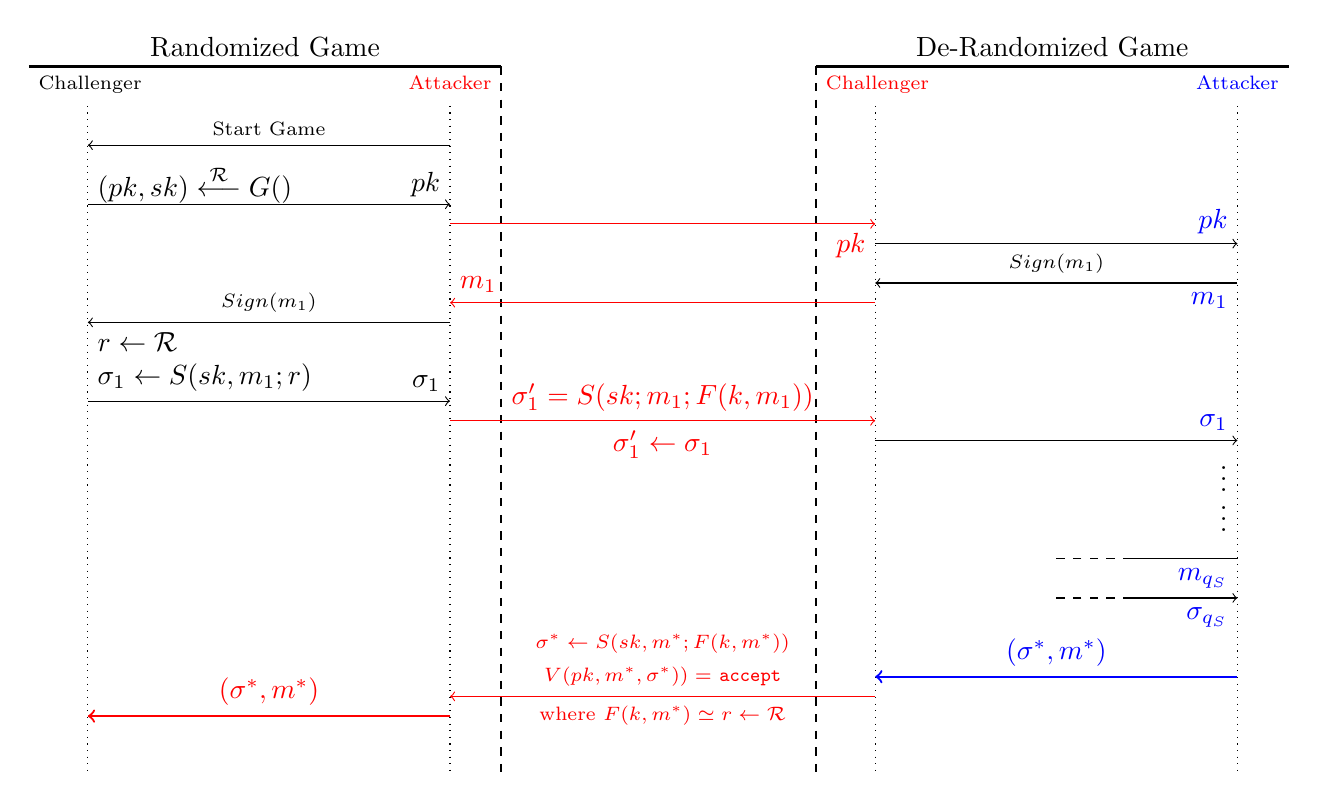
\begin{tikzpicture}
        % Define Variables
        \def\lR{0.75}
        \def\rR{5.35}
        \def\lDR{10.75}
        \def\rDR{15.35}
        \def\bottom{-9}

        % Overall Scheme
        \draw[thick] (0,0) -- (6,0) node[midway, anchor=south] {Randomized Game};
        \node[anchor = north west] at (0,0) (c-r) {\scriptsize Challenger};
        \draw[dotted] (\lR, -0.5) -- (\lR,\bottom);
        \node[anchor = north east, text=red] at (6,0) {\scriptsize Attacker};
        \draw[dotted] (\rR, -0.5) -- (\rR, \bottom);
        \draw[thick, dashed] (6,0) -- (6, \bottom);
        \draw[thick] (10,0) -- (16,0) node[midway, anchor=south] {De-Randomized Game};
        \node[anchor = north west, text=red] at (10,0) {\scriptsize Challenger};
        \node[anchor = north east, text=blue] at (16,0) {\scriptsize Attacker};
        \draw[thick, dashed] (10,0) -- (10, \bottom);
        \draw[dotted] (\lDR, -0.5) -- (\lDR, \bottom);
        \draw[dotted] (\rDR, -0.5) -- (\rDR, \bottom);

        % Start Games
        \draw[->] (\rR, -1) -- (\lR, -1) node[midway, anchor=south] {\scriptsize Start Game};
        \draw[->] (\lR, -1.75) -- (\rR, -1.75) node[midway, anchor=south] {};
        \node[anchor=west] at (\lR, -1.5) {$(pk, sk) \overset{\mathcal{R}}{\longleftarrow} G()$};
        \node[anchor=east] at (\rR, -1.5) {$pk$};
        \draw[->,color=red] (\rR, -2) -- (\lDR, -2) node[anchor=north east, text=red] {$pk$};
        \draw[->] (\lDR, -2.25) -- (\rDR, -2.25) node[anchor=south east, text=blue] {$pk$};

        % First Signing Query
        \draw[->] (\rDR, -2.75) -- (\lDR, -2.75) node[midway, anchor=south] {\scriptsize $Sign(m_1)$};
        \node[anchor=north east, text=blue] at (\rDR, -2.75) {$m_1$};
        \draw[->,color=red] (\lDR, -3) -- (\rR, -3) node[text=red,anchor=south west] {$m_1$};
        \draw[->] (\rR, -3.25) -- (\lR, -3.25) node[midway, anchor=south] {\scriptsize $Sign(m_1)$};
        \node[anchor=south west] at (\lR, -3.75) {$r \leftarrow \mathcal{R}$};
        \node[anchor=south west] at (\lR, -4.25) {$\sigma_1 \leftarrow S(sk,m_1;r)$};
        \draw[->] (\lR, -4.25) -- (\rR, -4.25) node[anchor=south east] {$\sigma_1$};
        \draw[->,color=red] (\rR, -4.5) -- (\lDR, -4.5) node[midway, anchor=south] {$\sigma_1' = S(sk;m_1;F(k, m_1))$} node[midway, anchor=north] {$\sigma_1' \leftarrow \sigma_1$};
        \draw[->] (\lDR, -4.75) -- (\rDR, -4.75) node[anchor=south east, text=blue] {$\sigma_1$};

        % Next Signing Queries
        \node[anchor=north east] at (\rDR, -4.75) {$\vdots$};
        \node[anchor=north east] at (\rDR, -5.25) {$\vdots$};
        \draw (\rDR, -6.25) node[anchor=north east, text=blue] {$m_{q_S}$} -- (14, -6.25);
        \draw[dashed] (14, -6.25) -- (13, -6.25);
        \draw[dashed] (14, -6.75) -- (13, -6.75);
        \draw[->] (14, -6.75) -- (\rDR, -6.75) node[anchor=north east, text=blue] {$\sigma_{q_S}$};

        % Forgery
        \draw[->, thick, color=blue] (\rDR, -7.75) -- (\lDR, -7.75) node[midway, anchor=south] {$(\sigma^*, m^*)$};
        \draw[->, thick, color=red] (\rR, -8.25) -- (\lR, -8.25) node[midway, anchor=south] {$(\sigma^*, m^*)$};
        \draw[->, color=red] (\lDR, -8) -- (\rR, -8) node[midway, anchor=south, text=red, align=center] {\scriptsize $\sigma^* \leftarrow S(sk, m^*; F(k, m^*))$ \\ \scriptsize $V(pk, m^*, \sigma^*)) = $ \texttt{accept}} node[midway, anchor=north, text=red] {\scriptsize where $F(k, m^*) \simeq r \leftarrow \mathcal{R}$};
        

    \end{tikzpicture}
    \caption{Attack scheme.\label{fig:attack-game}}
\end{figure}

Initially, the challenger in the randomized game, $C_R$, generates a keypair using it's randomized generator $G$ and sends $pk$ to the attacker (us).
We use the same $pk$ to initialize the de-randomized game against an attacker, $A_{DR}$, who is actually able to win the game.
Note that, in particular, we don't initialize the key for the PRF $F$.
This is an important observation as we will use our signing oracle in $C_R$ to model the randomness for $F$, and consequently answer signing queries to $A_{DR}$.

Once initialized, $A_{DR}$ performs a series of signing queries $Sign(m_1), \dots, Sign(m_{q_S})$.
For each query, he expects $\sigma_i' \leftarrow S'(sk', m_i) = S(sk, m_i; r') = S(sk, m_i; F(k, m_i)$.
We forward the query to $C_R$ and receive $\sigma_i \leftarrow S(sk, m_i; r)$ where $r \leftarrow \mathcal{R}$.
As $F$ is a secure PRF, no attacker has an advantage in telling whether the image he receives is the actually $F(k, m_i)$ for some $k \rightarrow R$, or it is a random value ($r \leftarrow R$).
Hence we send respond the query with $\sigma_i' = \sigma_i$.

Once $A_{DR}$ has finished querying, it outputs (by hypothesis) a valid forgery $(\sigma^*, m^*)$, which we can also send as a valid forgery to $C_R$ hence winning the randomized game, which was secure by construction.
This contradicts our initial assumption, hence $S'$ is indeed secure. \hfill $\qed$

\newpage
\section{Problem 4: Secret Sharing Schemes}\label{sec:problem4}

Let $p$ be a prime and let $q = p^r$ for some positive integer $r\in \Z ^+$.
Let $\P$ be a set of participants and $\Gamma \subset 2^\P$ be a monotone increasing access structure.

\begin{enumerate}
    \item Prove that if $\Gamma$ admits a vector space secret sharing scheme over $\F_p$, then $\Gamma$ admits a vector space secret sharing scheme over $GF(q)$.
    \item To prove that the opposite implication is not true, consider the threshold access structure for $n=4$ and $t=2$. Show that this access structure cannot admit a vector space secret sharing scheme over $F_2$, but it admits a vector space secret sharing scheme (which one?) over $GF(2^3)$.
\end{enumerate}

\begin{center}
    \rule{5cm}{0.4pt}
\end{center}

\textbf{\textit{Proof (1):}}
Since $\Gamma$ admits a vector space secret sharing scheme over $\F_p$, there exist $m\in \Z^+$ and $\psi : \P\cup \{D\} \to \F_p^m$ such that $A\in \Gamma$ if and only if $\psi(D)\in\langle \{\psi(P_j)\}_{P_j\in A}\rangle$.
Define
\begin{equation*}
    \begin{split}
        \Psi: \P\cup\{D\} &\longrightarrow (\F_p^m)^r\\
        P &\longmapsto (\psi(P),\ldots, \psi(P)).
    \end{split}
\end{equation*}
Suppose that we want to share a secret $S = (s_1, \ldots, s_r) \in GF(q)$.
Choose a random vector $v = (v_1, \ldots, v_r)\in (\F_p^m)^r$ satisfying $$v \cdot \Psi(D) = (v_1 \cdot \psi(D), \ldots, v_r \cdot \psi(D)) = (s_1, \ldots, s_r) = S,$$ and for $j = 1,\ldots, n$, let $S_j = v\cdot\Psi(P_j)$ be the piece of secret that each $P_j$ can compute.

If $A\in \Gamma$, by hypothesis we have that 
\begin{equation*}
    \begin{split}
        \psi(D) = \sum_{P_j\in A} \lambda^A_j \psi(P_j) \Rightarrow \Psi(D) = \sum_{P_j\in A} \lambda^A_j \Psi(P_j).
    \end{split}
\end{equation*}
Hence, the secret we wanted to share can be recovered by a linear combination of the pieces computed by the participants in $A$, 
\begin{equation*}
    \begin{split}
        \sum_{P_j \in A} \lambda^A_j S_j = \sum_{P_j \in A} \lambda^A_j v\cdot \Psi(P_j) = v\cdot (\sum_{P_j \in A} \lambda^A_j \Psi(P_j)) = v\cdot \Psi(D) = S.
    \end{split}
\end{equation*}

Observe that $(\F_p^m)^r \cong GF(q)^m$ because two finite fields of the same cardinality are isomorphic.
Via this isomorphism, it is clear that we can redefine $\Psi$ to have image in $GF(q)^m$.
Also, the coefficients $\lambda^A_j$ can be embedded in $GF(q)$ using the natural inclusion.

If $B\not \in \Gamma$, we want to see that the shares of participants in $B$ do not give any information about the secret.
The vector space secret sharing scheme over $\F_p$ satisfies that the probability of obtaining the pieces of the participants in $B$ is the same for any secret in $\F_p$.
Then, since $\psi(D) \not \in \langle \{\psi(P_j)\}_{P_j\in B}\rangle$ and by construction of $\Psi$, any possible secret in $GF(q)$ is also equally likely from the shares $\{S_j\}_{P_j\in B}$. 

Therefore, $\Gamma$ admits a vector space secret sharing scheme over $GF(q)$. \hfill $\qed$

\begin{center}
    \rule{5cm}{0.4pt}
\end{center}

\textbf{\textit{Proof (2):}}
Suppose that the $(2,4)$-threshold access structure, $\P = \{P_1, P_2, P_3, P_4\}$ and $\Gamma = \binom{\P}{2}$,  admits a vector space secret sharing scheme ove $\F_2$.
Let $\psi: \P \to \F_2^m$ be a map such that $A\in\Gamma$ if and only if $\psi(D)\in\langle \{\psi(P_j)\}_{P_j\in A}\rangle$, with $\psi(D) \in \F_2^m\setminus\{0\}$.
In particular, $\psi$ must satisfy
\begin{equation*}
    \begin{split}
        \psi(D) = & \lambda_1\psi(P_1) + \lambda_2\psi(P_2)\\
        \psi(D) = & \lambda_3\psi(P_2) + \lambda_4\psi(P_3)\\
        \psi(D) = & \lambda_5\psi(P_1) + \lambda_6\psi(P_3)
    \end{split}
\end{equation*}
for some $\lambda_i \in \F_2$.
In fact, $\lambda_i = 1 \forall i$ because a minimum of two participants is needed to recover the secret.
If we sum the first two equations, we get the contradiction $$0 = \psi(D) + \psi(D) = \psi(P_1) + \psi(P_3) = \psi(D).$$
Hence, the $(2,4)$-threshold access structure does not admit a vector space secret sharing scheme over $\F_2$.

To end, let us construct a vector space secret sharing scheme over $GF(8)$, as a counterexample of the opposite implication of the statement in (1).
First of all, recall that $GF(8)$ is the field of polynomials in $\F_2[x]$ of degree less than 3.
Define $\Psi : \P\cup\{D\} \to GF(8)^2$ by $\Psi(D) = (1, 0), \Psi(P_1) = (1, x), \Psi(P_2) = (1, x+1), \Psi(P_3) = (1, x^2), \Psi(P_4) = (1, x^2+1)$.
To satisfy the condition $A\in\Gamma$ if and only if $\Psi(D)\in\langle \{\Psi(P_j)_{P_j\in A}\}\rangle$, we have to solve
\begin{equation*}
    \begin{split}
        \Psi(D) = \lambda_{ij}\Psi(P_i) + \mu_{ij}\Psi(P_j), \text{ for } i < j.
    \end{split}
\end{equation*}
Let us compute the solution for our choice of $\Psi$:
\begin{equation*}
    \begin{split}
        \left.\begin{aligned}
        1 & = \lambda_{12} + \mu_{12}\\
        0 & = \lambda_{12} x + \mu_{12} (x+1)\\
        \end{aligned}\right\} & \iff \lambda_{12} = x + 1, \mu_{12} = x,\\
        \left.\begin{aligned}
        1 & = \lambda_{13} + \mu_{13}\\
        0 & = \lambda_{13} x + \mu_{13} x^2\\
        \end{aligned}\right\} & \iff \lambda_{13} = x^2+x+1,\mu_{13} = x^2+x,\\
        \left.\begin{aligned}
        1 & = \lambda_{14} + \mu_{14}\\
        0 & = \lambda_{14} x + \mu_{14} (x^2+1)\\
        \end{aligned}\right\} & \iff \lambda_{14} = x,\mu_{14} = x+1,\\
        \left.\begin{aligned}
        1 & = \lambda_{23} + \mu_{23}\\
        0 & = \lambda_{23} (x+1) + \mu_{23} x^2\\
        \end{aligned}\right\} & \iff \lambda_{23} = x^2+x,\mu_{23} = x^2+x+1,\\
        \left.\begin{aligned}
        1 & = \lambda_{24} + \mu_{24}\\
        0 & = \lambda_{24} (x+1) + \mu_{24} (x^2+1)\\
        \end{aligned}\right\} & \iff \lambda_{24} = x^2,\mu_{24} = x^2+1,\\
        \left.\begin{aligned}
        1 & = \lambda_{34} + \mu_{34}\\
        0 & = \lambda_{34} x^2 + \mu_{34} (x^2+1)\\
        \end{aligned}\right\} & \iff \lambda_{34} = x^2+1,\mu_{34} = x^2.\\
    \end{split}
\end{equation*}
To share a secret $s \in GF(8)$, we have to choose a random vector $v\in GF(8)^2$ such that $v\cdot\Psi(D) = s$.
Each participant $P_j$ is able to compute $s_j = v\cdot \Psi(P_j)$, and the secret can be recovered using the computed coefficients, 
\begin{equation*}
    \begin{split}
        s = \lambda_{ij}s_i + \mu_{ij}s_j,
    \end{split}
\end{equation*}
for each pair $(i,j)$ with $i<j$.
Observe that only one participant does not give any information about the secret.

This vector space secret sharing scheme is the well-known Shamir secret sharing scheme.
For a general $(t, n)$-threshold access structure and a finite field $\F$ with more than $n$ elements, we have to choose $n$ different elements $\alpha_1,\ldots,\alpha_n \in \F\setminus\{0\}$, and define $\Psi(D) = (1,0, \ldots, 0)$, $\Psi(P_i) = (1, \alpha_i, \ldots, \alpha_i^{t-1})$. \hfill $\qed$



\end{document}
